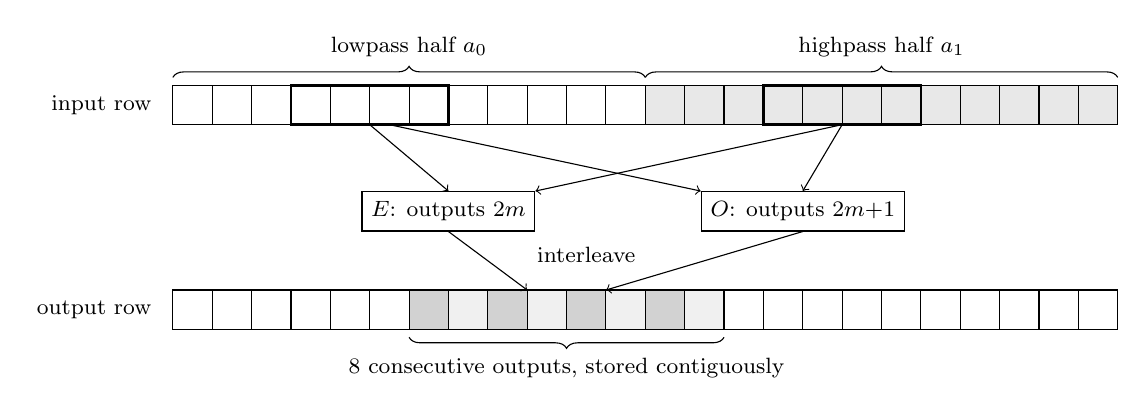
\begin{tikzpicture}[x=0.5cm,y=-0.5cm,font=\footnotesize]
  % input row: lowpass half then highpass half
  \foreach \i in {0,...,11} \draw (\i,0) rectangle (\i+1,1);
  \foreach \i in {12,...,23} \draw[fill=gray!18] (\i,0) rectangle (\i+1,1);
  \node[anchor=east] at (-0.3,0.5) {input row};
  \draw[decorate,decoration={brace,amplitude=4pt}] (0,-0.2) -- (12,-0.2) node[midway,above=4pt] {lowpass half $a_0$};
  \draw[decorate,decoration={brace,amplitude=4pt}] (12,-0.2) -- (24,-0.2) node[midway,above=4pt] {highpass half $a_1$};
  % a vector of 4 consecutive m in each half
  \draw[line width=1pt] (3,0) rectangle (7,1);
  \draw[line width=1pt] (15,0) rectangle (19,1);
  % even and odd vectors
  \node[draw,minimum width=2cm,minimum height=5mm] (E) at (7,3.2) {$E$: outputs $2m$};
  \node[draw,minimum width=2cm,minimum height=5mm] (O) at (16,3.2) {$O$: outputs $2m{+}1$};
  \draw[->] (5,1) -- (E.north);
  \draw[->] (17,1) -- (E.north east);
  \draw[->] (5.5,1) -- (O.north west);
  \draw[->] (17,1) -- (O.north);
  % interleaved output
  \foreach \i in {0,...,23} \draw (\i,5.2) rectangle (\i+1,6.2);
  \foreach \i in {6,8,...,12} \fill[gray!35] (\i,5.2) rectangle (\i+1,6.2);
  \foreach \i in {7,9,...,13} \fill[gray!12] (\i,5.2) rectangle (\i+1,6.2);
  \foreach \i in {6,...,13} \draw (\i,5.2) rectangle (\i+1,6.2);
  \node[anchor=east] at (-0.3,5.7) {output row};
  \draw[->] (E.south) -- (9,5.2);
  \draw[->] (O.south) -- (11,5.2);
  \node at (10.5,4.3) {interleave};
  \draw[decorate,decoration={brace,amplitude=4pt,mirror}] (6,6.4) -- (14,6.4) node[midway,below=4pt] {8 consecutive outputs, stored contiguously};
\end{tikzpicture}
